\documentclass{standalone}
\usepackage{tikz}
\usetikzlibrary{arrows.meta}

\begin{document}
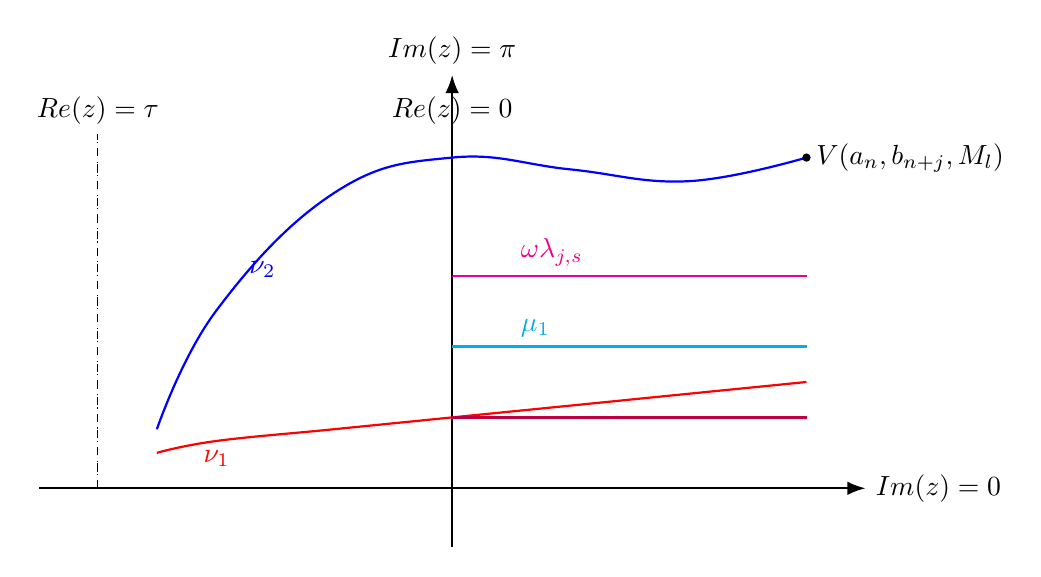
\begin{tikzpicture}[scale=1.5]

% Axes
\draw[thick, -Latex] (-3.5, 0) -- (3.5, 0) node[right] {$\operatorname{Im}(z)=0$};
\draw[thick, -Latex] (0, -0.5) -- (0, 3.5) node[above] {$\operatorname{Im}(z)=\pi$};

% Dashed lines for Re(z) = \tau and Re(z) = 0
\draw[dashed] (-3, 0) -- (-3, 3) node[above] {$\operatorname{Re}(z)=\tau$};
\draw[dashed] (0, 0) -- (0, 3) node[above] {$\operatorname{Re}(z)=0$};

% Curves
\draw[blue, thick] plot[smooth, tension=0.7] coordinates {(-2.5, 0.5) (-2, 1.5) (-1, 2.5) (0, 2.8) (1, 2.7) (2, 2.6) (3, 2.8)};
\node[blue, anchor=south west] at (-1.8, 1.7) {$\nu_2$};

\draw[red, thick] plot[smooth, tension=0.7] coordinates {(-2.5, 0.3) (-2, 0.4) (-1, 0.5) (0, 0.6) (1, 0.7) (2, 0.8) (3, 0.9)};
\node[red, anchor=north east] at (-1.8, 0.4) {$\nu_1$};

\draw[magenta, thick] plot[smooth, tension=0.7] coordinates {(0, 1.8) (1, 1.8) (2, 1.8) (3, 1.8)};
\node[magenta, anchor=south west] at (0.5, 1.8) {$\omega\lambda_{j,s}$};

\draw[cyan, thick] plot[smooth, tension=0.7] coordinates {(0, 1.2) (1, 1.2) (2, 1.2) (3, 1.2)};
\node[cyan, anchor=south west] at (0.5, 1.2) {$\mu_1$};

\draw[purple, thick] plot[smooth, tension=0.7] coordinates {(0, 0.6) (1, 0.6) (2, 0.6) (3, 0.6)};

% Labels for V(a_n, b_{n+j}, M_l)
\fill[black] (3, 2.8) circle (1pt);
\node[right] at (3, 2.8) {$V(a_n, b_{n+j}, M_l)$};

% Annotations
\foreach \x in {-3, 0} {
    \draw[dotted] (\x, 0) -- (\x, 3);
}

\end{tikzpicture}
\end{document}